\chapter{Results}\label{c3}

\section{Overall results}

\autoref{t4} shows the overall results obtained when the criterion hyperparameter is optimised for DT and RF, and the weights hyperparameter is optimised for kNN through five-fold cross-validation, using both imbalanced and balanced training data. The optimal hyperparameter is the one that produces the highest average F1 score. For each classification performed, the optimal hyperparameters were found to be the non-default values. The mean and standard deviation were obtained by averaging all scores output by all turbines for the optimal hyperparameter. From these results, all three classifiers performed better, with higher mean and lower standard deviation scores, when trained on imbalanced datasets using the multilabel classification approach compared to balanced datasets with separate estimators for each label. The F1 scores for DT, RF and kNN is higher by 0.6\,\%, 0.5\,\% and 1.9\,\% respectively using imbalanced data compared to balanced data. The best performance was by RF using imbalanced data, which had the highest mean and lowest deviation scores. The kNN classifier meanwhile produced the results with the lowest mean and highest deviations. An attempt was made to further improve the performance of RF by optimising the number of estimators hyperparameter, but this was not possible as the process was found to exceed the available RAM. Hence, the only hyperparameter considered for further tuning is the k value for kNN using imbalanced dataset. The default value of k is 5 on scikit-learn, and values between 1 and 200 were tested. \autoref{f3} shows the optimal k values found for each turbine, which are the values that produce the highest average F1 score. The optimal k is 13 or less for 17 turbines, and more than 100 for 5 turbines. Based on the overall scores in \autoref{t4}, the optimisation did increase the F1 score of kNN by 0.6\,\% compared to using the imbalanced data without k optimisation, but compared to the F1 scores of DT and RF using imbalanced data, this is still lower by 5.1\,\% and 6.1\,\% respectively.

\begin{table}
  \centering
  \caption{\label{t4}Overall precision, recall and F1 scores for optimising hyperparameters for decision trees and random forests, and k nearest neighbours. The mean and standard deviation are obtained by averaging all scores output by all turbines for the optimal hyperparameter. The values are colour-coded to show better performances (i.e., higher mean and lower standard deviation) in darker shades and worse performances in lighter shades.}
  \includegraphics[width=\textwidth]{../images/t4}
\end{table}

\begin{figure}
  \centering
  \includegraphics[width=.9\textwidth]{../images/f3}
  \caption{\label{f3}Number of neighbours, or k value for each turbine optimised based on the average F1 score through five-fold cross-validation. The optimal k is 13 or less for 17 turbines, and more than 100 for 5 turbines.}
\end{figure}

The time taken to execute the Python code using the optimal hyperparameters to produce the results for all 25 turbines, which includes reading the merged CSV file, processing and labelling samples, classification using cross-validation, and calculation of performance metrics, for each classifier is listed in \autoref{t5}. As other processes running in the background at the time of execution and some runs were interrupted due to computer crashes, the time taken could not be measured accurately and these values are only approximate. Overall, balancing the training data is shown to increase the training time, which is expected as the size of training data will be larger and separate estimators are used for each label compared to just one when using imbalanced data. DT and RF only took 8 hours with imbalanced data. Despite balancing the training data, DT and RF took only 18 hours compared to kNN with imbalanced data, which took 20 hours. The relatively long timings make kNN an inefficient classifier compared to DT and RF. As a result, the following results will only focus on the classifier with the best performance, which is RF. The other classifiers, however, can be tested more efficiently if better computing resources are available.

\begin{table}
  \centering
  \caption{\label{t5}Time taken to run each classifier using imbalanced and balanced datasets for the 30-month period. These timings are approximate as the RAM was not utilised fully by the Python application due to other processes running in the background, and the application had to be restarted a number of time due to system crashes.}
  \includegraphics{../images/t5}
\end{table}

\section{Performance of each turbine and label}

The classification results using random forests for each turbine and label in full can be found in \autoref{a3}. The scores of each performance metric from cross-validation were grouped based on turbine or label which were then averaged to produce the mean scores. Additionally, the maximum and minimum values were also found. The turbine with the worst performance is turbine 1, with a mean and minimum F1 scores of 87\,\% and 44\,\% respectively using imbalanced data, and 86\,\% and 41\,\% respectively using balanced data, for turbine 1. Four other turbines had minimum scores less than 70\,\%, namely turbines 7, 9 ,15 and 16. Looking at the labels, turbine category 10, which is `electrical system' had the worst performance, with mean and minimum F1 scores of 84\,\% and 44\,\% respectively using imbalanced data, and 82\,\% and 41\,\% respectively using balanced data. These minimum scores correspond to the scores for turbine 1. Therefore, it can be deduced that the classifier's ability to predict faults in the electrical system is relatively low. This is followed closely by turbine category 11, `pitch control', which has mean and minimum F1 scores of 84\,\% and 57\,\% respectively using imbalanced data and 83\,\% and 55\,\% respectively using balanced data. For all other turbine categories, the minimum score did not drop below 75\,\%.

\autoref{f4} shows the various turbine categories quantified by downtime frequency on the left and period on the right, both per turbine per year. Looking at only turbine categories used as labels, `pitch control' and `electrical system' are the two categories causing the most downtime events and are in the top three in terms of the downtime period. These two labels also had the worst performance scores.

\begin{figure}
  \centering
  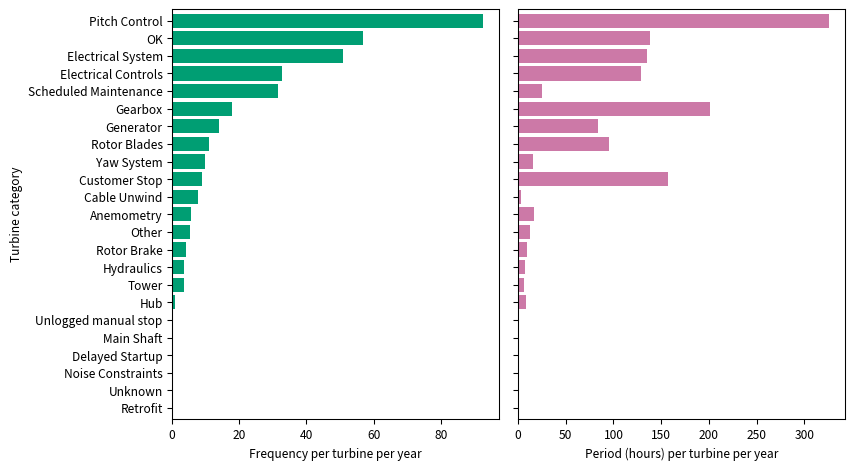
\includegraphics[width=\textwidth]{../images/f4}
  \caption{\label{f4}Bar chart showing the various turbine categories quantified by the downtime frequency per turbine per year on the left, and downtime period, in hours, per turbine per year on the right. This was plot using the downtime data.}
\end{figure}

\section{Performance of each class}

Since turbine category 10 was found to have the worst performance, the performance of each class for this label is looked at in more detail, which is done by obtaining confusion matrices. A confusion matrix displays, for each class, the number of samples predicted correctly and what the wrongly predicted samples were classified as \cite{33M}. This will allow the decision to be made whether the number of classes and intervals used for fault prediction can be tweaked for better classifier performance. The matrices were first obtained for all turbines with only this label using both imbalanced and balanced training data. Through five-fold cross-validation, a total of 125 matrices were produced, which were then combined and normalised, which will produce the classification accuracy. The confusion matrices are shown in \autoref{a4}. 93-95\,\% of `normal' and 73-75\,\% of `curtailment' samples were classed correctly. In comparison, only 21-24\,\% of `faulty' samples were classified correctly, with 47-48\,\% misclassified as `curtailment' and 21-26\,\% misclassified as `normal'.

Due to this misclassification percentage being higher than the accuracy of the `faulty' class, the classification was repeated by dropping all rows with `curtailment', effectively removing the class. There is a significant improvement in the accuracy of `faulty' samples, from 21-24\,\% to 41-44\,\%. However, the majority of samples belonging to this class (44-49\,\%) were still misclassified as `normal'. In fact, this is the case for the `X hours before fault' classes, with or without the use of the `curtailment' class. As X increases, the accuracy is seen to decrease, and the percentage of misclassification as `normal' increases.

To make a comparison, the same analysis was repeated for turbine category 5, which is `gearbox'. This category was chosen as its mean F1 score was relatively high (92\,\% compared to 84\,\% for turbine category 10), it causes the second longest downtime period based on \autoref{f4}, and it indicates a problem in the mechanical system, rather than electrical. 96-97\,\% of `normal' and 83\,\% of `curtailment' samples were classed correctly. In comparison, 43-44\,\% of `faulty' samples were classified correctly, with 16-21\,\% misclassified as `curtailment' and 34-40\,\% misclassified as `normal'. The performance was better compared to turbine category 10, but the misclassification of the `faulty' class as `normal' is higher. Removing the `curtailment' increased the accuracy of `faulty' samples, from 43-44\,\% to 48-55\,\%. However, the misclassification of this class as `normal' was still high (41-48\,\%).

Using a balanced dataset overall decreased the misclassification rate of `X hours before fault' classes as `normal', but increased the misclassification of the `faulty' class as `normal'.

\section{Feature importance}

The importance of each feature used, which are a set of normalised scores \cite{Rudy13}, were also obtained similar to the confusion matrix. The higher the feature importance, the more influence the feature had in determining the class of the samples. The feature importance for turbine categories 10 and 5 are shown in \autoref{t6}. For both turbine categories, the wind speed and nacelle position were found to be the most important features, and the maximum, average and deviations of the active power were found to be the least important, regardless of training data balancing. The wind direction was the third most important feature for turbine category 10 regardless of balancing, and for turbine category 5 using imbalanced data. In the case of balanced data for turbine category 5, the third most important feature was the pitch angle.

\begin{table}
  \centering
  \caption{\label{t6}Feature importance for turbine categories 10 and 5 using random forests and either imbalanced (I) or balanced (B) training data. The values are normalised and colour-coded, transitioning from red (lower importance) to yellow (intermediate) to green (higher importance).}
  \includegraphics[width=\textwidth]{../images/t6}
\end{table}
